\documentclass[12pt]{article}
\usepackage[top=1in, bottom=1in, left=1in, right=1in]{geometry}
\parindent 22pt

\usepackage{adjustbox}
\usepackage{amsmath}
\usepackage{amssymb}
\usepackage{array}
\usepackage{booktabs}
\usepackage{datetime}
\usepackage{fancyhdr}
\usepackage{float}
\usepackage{graphicx}
\usepackage[colorlinks=true,linkcolor=blue,urlcolor=blue,anchorcolor=blue,citecolor=blue]{hyperref}
\usepackage{lscape}
\usepackage{multirow}
\usepackage{natbib}
\usepackage{setspace}
\usepackage{tabularx}
\usepackage[colorinlistoftodos,linecolor=black]{todonotes}
\usepackage{appendix}
\usepackage{pgffor}
\usepackage{caption} 
\usepackage{threeparttable}
\captionsetup[table]{skip=3pt}

\settimeformat{hhmmsstime}

\newcolumntype{L}[1]{>{\raggedright\arraybackslash}p{#1}}
\newcolumntype{C}[1]{>{\centering\arraybackslash}p{#1}}
\newcolumntype{R}[1]{>{\raggedleft\arraybackslash}p{#1}}


\begin{document}

\title{Estimation of the Effects of the Reggio-Approach Infant-Toddler Centers}
\author{Reggio Team}
\date{Original version: September 1, 2016 \\ Current version: \today}
\maketitle

\doublespacing

\section{Introduction}
In this document, we focus on estimating treatment effects of the Reggio-Approach infant-toddler centers. We begin by providing the current background information we have on evolution of infant-toddler centers in Italy and infant-toddler centers in different cities. We discuss the types of infant-toddler centers attended in the data and their basic statistics. Estimation methods, which reflect the evolution and curricula of infant-toddler centers across Reggio, Parma, and Padova, are presented.


\section{Background}
\subsection{Evolution of Infant-Toddler Centers in Italy}
The Italian child care system is divided in infant-toddler centers (asilo) for children aged 0-3, and preschool (materna) for children aged 3-6. Infant-toddler centers are provided mainly by the municipalities and private institutions in more limited supply than preschools. While the number of preschools for ages 3-6 increased rapidly over the years, the number of infant-toddler centers remained very low. 


%\begin{table} \caption{History of Infant-Toddler Centers in Italy}
%\begin{tabular}{ll}
%\toprule
%\textbf{}

%\end{tabular}
%\end{table}


Only under \textbf{the 2002 Budget} (Law N. 448 dated 2001/12/28) infant-toddler centers were defined as services able to improve the education and the socialization of children; in some regions, like Toscana, Emilia Romagna and Liguria, new legislation was proposed in which infant-toddler centers were considered ``educational" and not merely an instrument for reconciling family and work, or to support the disadvantaged. The 2002 Budget (and the subsequent 2003 and 2004 Budgets) foresaw the transfer of funds from the State to the regional authorities for the extension and the improvement of the existing infant-toddler centers throughout the country, above all in view of the Lisbon Objectives. 

The European Union began to declare the importance of supplying accessible child care for ages 0-3 as policy to encourage female employment in 1992 and in 2002, during the Barcelona summit, set the objective (to be reached by 2010) at 33\% of all children under the age of three. It is important to emphasize that the European Commission not only introduced this quantitative target on the availability of infant-toddler centers, but also produced successive documents emphasizing the qualitative aspects: infant-toddler centers should contribute to the emotional, social, and cognitive development of the child. 

\textbf{The 2007-2008 Budgets} were extraordinary measures approved for the extension of childcare services for ages 0-3. The transfer of funds from the State to the regional authorities was foreseen, with the following division of duties regarding the infant-toddler centers: the regions are responsible for the allocation of the resources made available by the State for the lower levels of government; the provincial authorities are responsible for the supervisory activities and the training of the teachers; the local councils are responsible for managing the existing infant-toddler centers, carrying out maintenance and building work and eventually opening new ones (financed by them). This division of duties is still in force and, importantly, the criteria for the opening and management of new infant-toddler centers vary according to the region, as do the criteria for admission. 


\subsection{Infant-Toddler Centers in Different Cities}
\subsubsection{Reggio Emilia}
The Reggio Approach infant-toddler centers are the oldest childcare system in Italy. It started in 1971 with the opening of the first municipal infant-toddler center in Reggio Emilia, and this was earlier than the 1971 National Law. Infant-toddler centers in Reggio Emilia accommodate infants aged from 3 months to 3 years. 

In Reggio Emilia, the municipal infant-toddler centers open at 8 am. Families can choose three options for pick-up: 1 pm (part-day), 4 pm (full-time), and until 6:20 pm (extended day). Teachers in the infant-toddler centers generally have lower initial training and receive less pay. The atelier and role of atelierista is not part of the infant-toddler center program, but in Reggio-Approach centers, teachers are trained by atelieristas from the older schools. In contrast to the Reggio-Approach age 3-6 preschools, teachers in the infant-toddler centers are assigned to children in single year increments.  

\subsubsection{Parma}
The first infant-toddler centers in Parma were opened in 1975 after the 1971 National Law. Infant-toddler centers in Parma accommodate infants aged from 5 months to 3 years. As of 2001, 16 infant-toddler centers were offered throughout the municipality. The administration of these centers are managed by a City Director of Services for Children. 

Infant-toddler centers in Parma have pedagogical coordinators, who perform both administrative and professional development roles. Assigned to a specific set of infant-toddler centers, they meet twice each month with all site teachers collectively for shared reflection, on-site supervision, and promotion of relationships with families. The City Director meets biweekly with all pedagogical coordinators for overall planning. University professors or administrators from other municipalities provide professional development in the form of continuing education. (Terzi and Cantarelli, 2001)

Parma's infant-toddler centers are intentionally designed in the context of an apartment. Terzi and Cantarelli report mixed-age classes that include 18 total children from 13 - 36 months in a single section, led by 2 teachers, for a 1:9 teacher-child ratio. The infant-toddler centers open at 7:30 am and have three options for pick-up times: 2 pm (short-day), 3:30 pm (normal day), and 5 pm (extended day).


\subsubsection{Padova}
The first infant-toddler centers in Padova were opened in 1976 after the 1971 National Law. 

In 1989, the region of Veneto reported a total provision of childcare slots for 3.9\% of its infant-toddler population. The practice of professional development trainings for early childhood staff in Veneto first began in 1986.



\section{Data}

\begin{landscape}
\begin{figure}
\caption{Type of Infant-Toddler Center Attended, by City and Cohort}
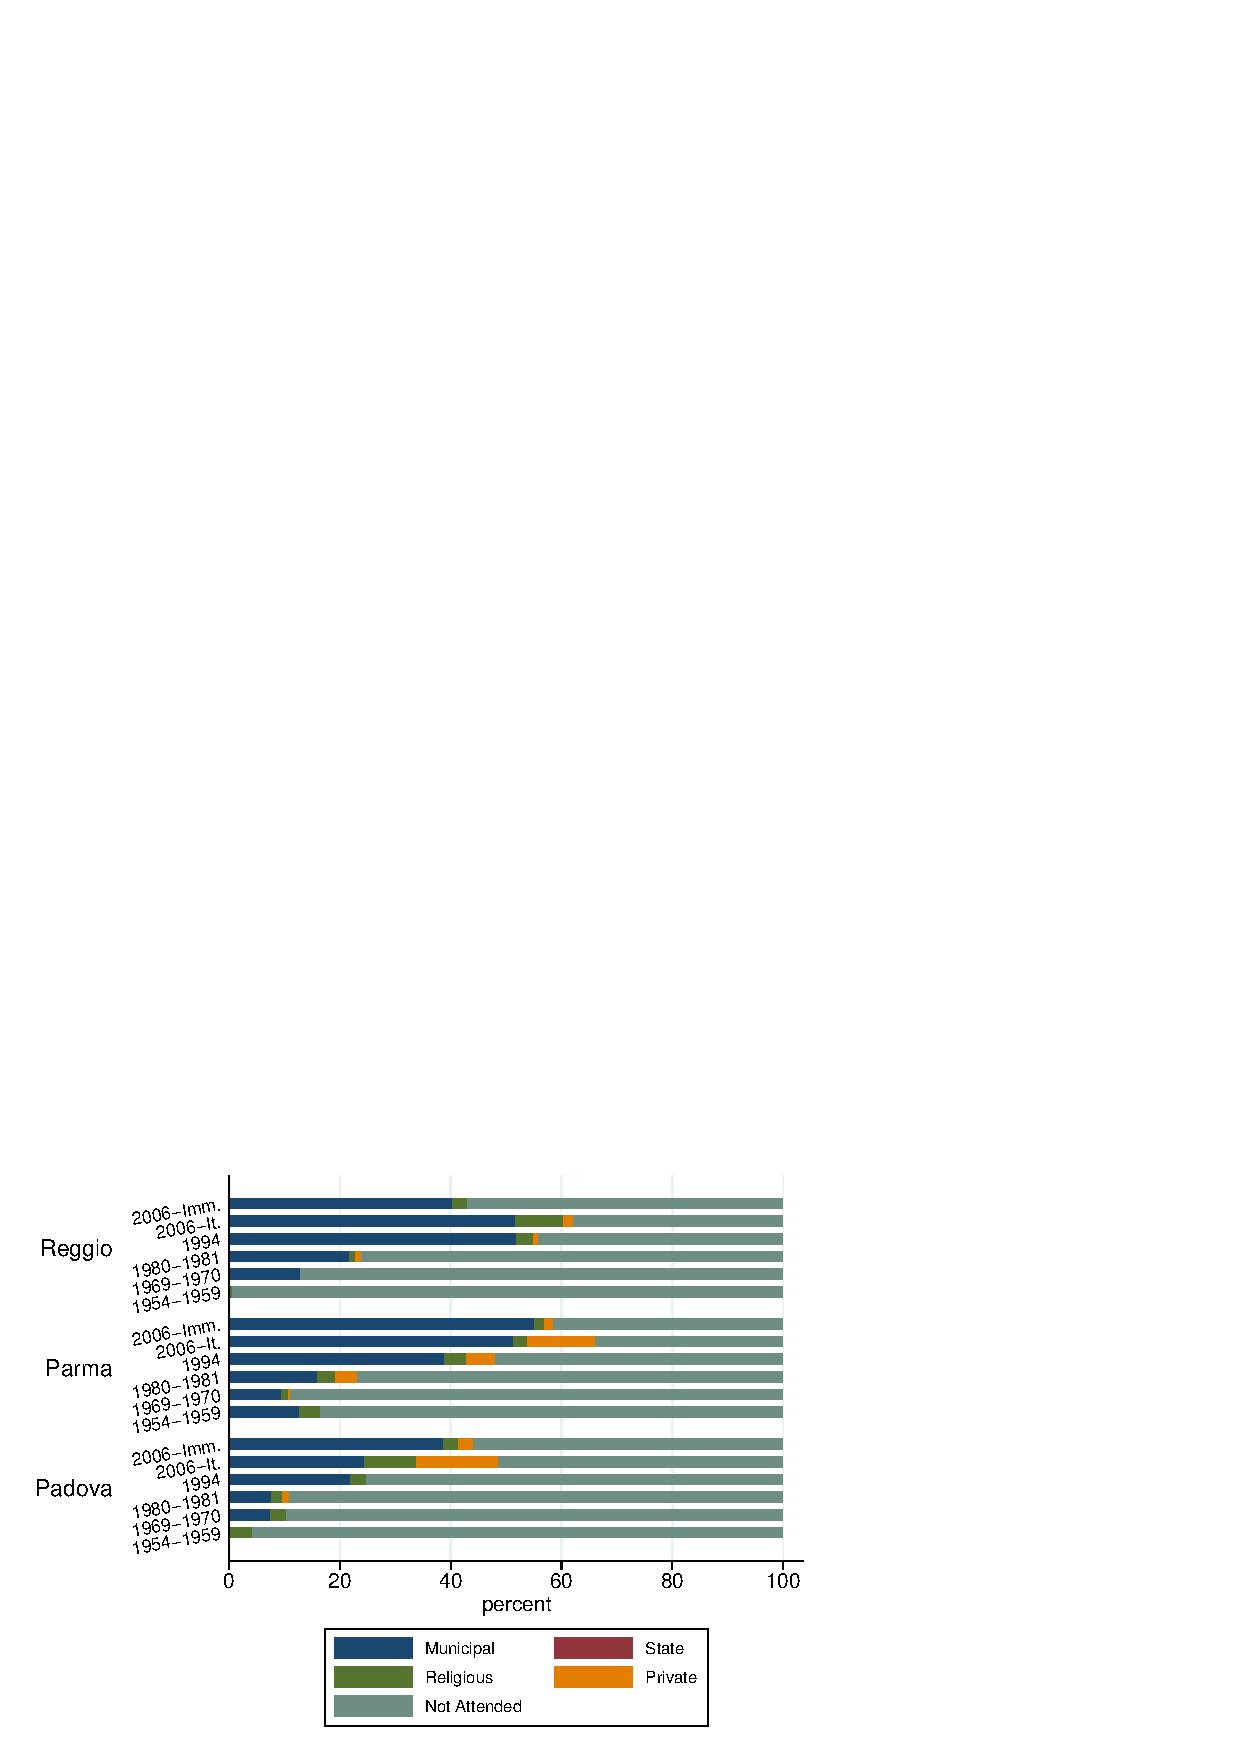
\includegraphics[scale=0.7]{../../../../output/image/asiloType-Attend.png} 
\end{figure}
\end{landscape}

\end{document}
